\subsection{Testbericht Backend}\label{backendTestbericht}
Das Backend wurde isoliert von der Android-App manuell getestet. Zu diesem Zweck wurde Swagger verwendet. Swagger stellt eine Bedienoberfläche bereit, mit welcher man alle Funktionen der Travelbuddy API testen kann. Um das Backend testen zu können, mussten vorher Beispiel-Daten erfasst werden. Diese wurden ebenfalls für das Testen der Android-App und Demozwecke verwendet. Da wir keine Applikation zum Erfassen von Touren entwickeln, mussten die Daten direkt über die SQL-Datenbank erfasst werden. Beim Testen der API wurde jede einzelne Funktion aufgerufen und überprüft, ob das korrekte Resultat vom Backend zurückgegeben wurde. System- und Integrationstests wurden dadurch im Selben durchgeführt. Denn diese Tests gaben Aufschluss darauf, ob die Kommunikation mit der Google-Maps API und der Datenbank richtig funktionierten. Einfachheitshalber haben wir auf ein Ticketing-System verzichtet. In Zukunft müssten aber die Issues in einem System verwaltet werden. In diesem Stadium des Projekts war dies allerdings nicht nötig. Fehler die von den Android-App-Entwickler entdeckt wurden, haben diese direkt an die Backend-Entwickler via Slack kommuniziert. Diese Kommunikation funktionierte gut und dadurch konnte sehr rasch auch auf Änderungswünsche bezüglich der API eingegangen werden.

Um bei Änderungen oder Erweiterungen am Backend sicher zu sein, dass die bestehende Funktionalität nicht negativ beeinflusst wurde, haben wir für die wichtigsten Funktionen Unit-Tests geschrieben. Nachfolgend einer Zusammenfassung der umgesetzten Unit-Tests und deren Testresultat. Zum Zeitpunkt des Code-Freeze am 15. Mai 2017 laufen alle Unit-Tests erfolgreich durch.

\begin{figure}
  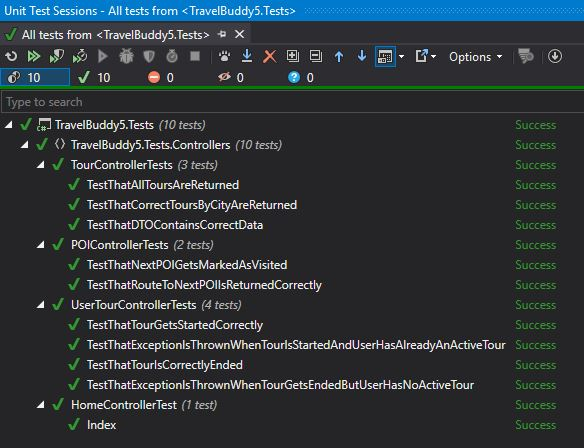
\includegraphics{backend_unit_test_summary}
  \caption{Unit-Test-Bericht Backend }
\end{figure}
